\documentclass{anstrans}
%%%%%%%%%%%%%%%%%%%%%%%%%%%%%%%%%%%
\title{}
\author{Baptiste Mouginot,$^{*}$ Kathryn Mummah,$^{*}$ Paul P.H. Wilson$^{*}$}

\institute{
$^{*}$University of Wisconsin-Madison, WI
}

\email{mouginot@wisc.edu \and mummah@wisc.edu \and paul.wilson@wisc.edu}

% Optional disclaimer: remove this command to hide
% \disclaimer{Notice: this manuscript is a work of fiction. Any resemblance to
% actual articles, living or dead, is purely coincidental.}

%%%% packages and definitions (optional)
\usepackage{graphicx} % allows inclusion of graphics
\usepackage{booktabs} % nice rules (thick lines) for tables
\usepackage{microtype} % improves typography for PDF
\usepackage{float}

\newcommand{\SN}{S$_N$}
\renewcommand{\vec}[1]{\bm{#1}} %vector is bold italic
\newcommand{\vd}{\bm{\cdot}} % slightly bold vector dot
\newcommand{\grad}{\vec{\nabla}} % gradient
\newcommand{\ud}{\mathop{}\!\mathrm{d}} % upright derivative symbol


\usepackage[acronym]{glossaries}
\newacronym{UOX}{UOX}{uranium oxide fuel}
\newacronym{MOX}{MOX}{mixed oxide fuel}
\newacronym{LWR}{LWR}{light water reactor}
\newacronym{FBR}{FBR}{fast breeder reactor}

\begin{document}
%%%%%%%%%%%%%%%%%%%%%%%%%%%%%%%%%%%%%%%%%%%%%%%%%%%%%%%%%%%%%%%%%%%%%%%%%%%%%%%%
\section{Introduction}

Fuel cycle simulations, as any simulation process, do not produce results
without errors. Those errors have different sources: data uncertainties (when
the simulation relies on previously estimated/measured metrics), modeling
uncertainties (produced by the simplification made by the simulator) and the
``functional`` uncertainty (uncertainty on the operation parameters of the
different facilities).

Some treaty verification scenarios require estimating historical fissile
material production based on records of facility operation and material
transfer.  If the measurements of facility operation and material transfer are
subject to uncertainty, the total production quantities will then also be
uncertain, creating an opportunity for undetected diversion.  This study seeks
to understand which measures of facility operation have the most impact on the
uncertainty of fissile material production across a complete fuel cycle.  A
``Total Monte Carlo'' approach will be applied to the Cyclus fuel cycle simulator
\cite{cyclus} to estimate output metrics uncertainty caused by individual
facility uncertainties.

\section{Method}

To estimate the uncertainty on fuel cycle output metrics, a ``Total Monte
Carlo'' approach has been applied. In the following, output metric uncertainty
corresponds to the Standard Deviation of the output metrics over about 200
different simulations. For each uncertainty associated parameter, an
artificially large uncertainty of $10\%$ have been Normally distributed.

To pursuit this work, both the Cycamore\cite{cycamore} package and the
CyCLASS\cite{cyclass} have been updated to deal with uncertainty in different
operational parameters of their different facility.  Table
\ref{tab:package_uncertainty} summarize all the modification implemented in the
different facilities present in Cycamore and CyCLASS.


\begin{table}[htb]
\centering
  \caption{Summary of facility modification per source package.}
\begin{tabular}{cll}
\toprule

Package   & Facility   & Parameters                \\
\midrule
Cycamore & Enrichment & Tail Assay                \\
         & Separation & Separation efficiency     \\
         & Storage    & Residence Time            \\
\midrule
CyCLASS  & Reactor    & Cycle Length              \\
         &            & Power                     \\
         &            & Fuel Enrichment (PWR-UOX) \\

\bottomrule
\end{tabular}

  \label{tab:package_uncertainty}
\end{table}

\section{The Experiment}
\subsection{The Fuel Cycle}
This work aims to assess the impact of the functional uncertainties of a
simple transition (see Figure \ref{fig:cycle}) inspired from the EG23 of the Screening And
Evaluation Group\cite{FCO}: a transition from light water reactors fleet loaded
with \glspl{UOX} fuel to a sodium fast reactors fleet loaded \glspl{MOX} fuel, considering an
$1\%/$y grows of the generated power (Figure \ref{fig:power}).
\begin{figure}[ht] % replace 't' with 'b' to force it to be on the bottom
  \centering
  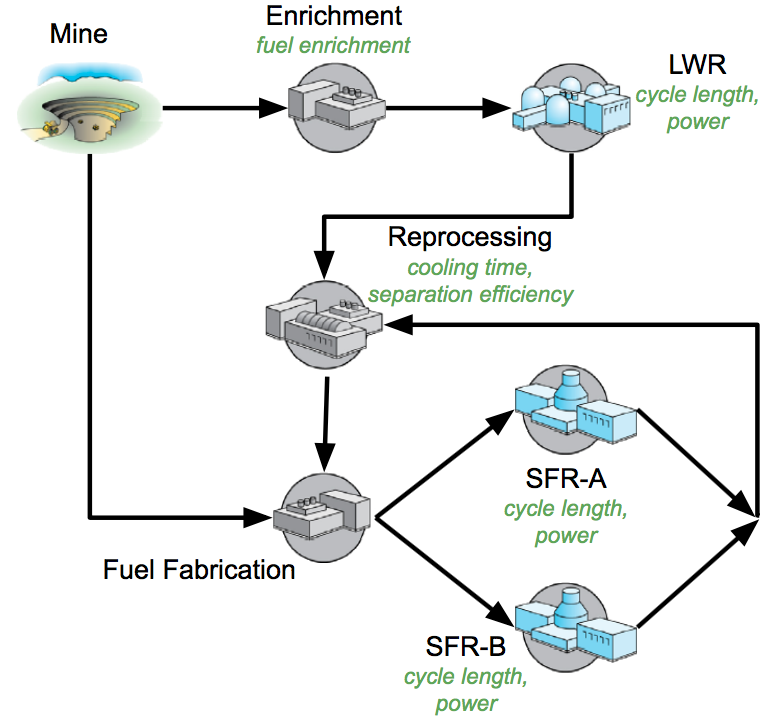
\includegraphics[scale=0.31]{cycle.png}
  \caption{Illustration of the material flow between the different facilities,
  with in green each operational parameters associated with an
  uncertainty.}\label{fig:cycle}
\end{figure}

As illustrated on Figure \ref{fig:power}, the transition starts with a fleet
fully composed by \glspl{LWR} loaded with enriched \glspl{UOX} fuel. The actual
transition starts around year 35, with the deployment of \glspl{FBR}, loaded
with Mixed oxide fuel (MOX), consisting of plutonium blended with natural
uranium. Once the transition to a full \glspl{FBR} fleet is completed, the
\glspl{FBR} fleet is slowly replaced with \glspl{FBR} with a lower breeding
ratio. 

\begin{figure}[ht] % replace 't' with 'b' to force it to be on the bottom
  \centering
  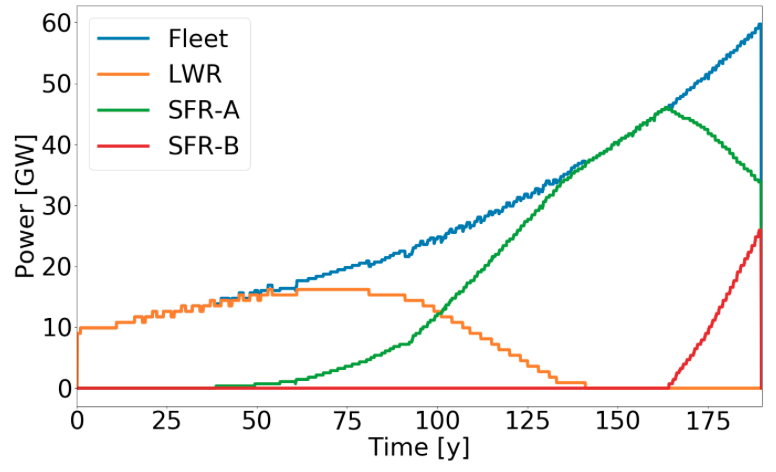
\includegraphics[scale=0.32]{power.png}
  \caption{Electric power generated over time, with in blue the full production,
      in orange the \glspl{LWR} contribution, in green the hight breeding ratio
    \glspl{FBR} and in red the low breeding ratio \glspl{FBR}.}
    \label{fig:power}
\end{figure}


The plutonium, required for the \glspl{MOX} fabrication, is reprocessed
from all used fuel, at first only used UOX, then used MOX fuel as they start to
be available for reprocessing.

Both fuel reprocessing and fabrication are done at a constant rate (constrained
by the feed materials availabilities). The enrichment of the UOX is processed on
demand. Buffer storages (not shown on Figure \ref{fig:cycle}) is present between
all facilities with constant processing rates.

\subsection{Uncertainty Measurements}
In this specific study, one will only focus on the uncertainty on the produced
electric power as a function of time, on the total quantity of natural uranium
used and on the total unused fissile inventory (unused reprocessed plutonium).
In order to estimate the total uncertainty on those 3 parameters as well as the
individual contribution of the operational parameters several set of (199) simulations
have been completed.

In addition to the set with all parameters are sampled according to their
uncertainty, a set a have been computed for each parameter, with all the other
remaining fixed to the reference value.



%%%%%%%%%%%%%%%%%%%%%%%%%%%%%%%%%%%%%%%%%%%%%%%%%%%%%%%%%%%%%%%%%%%%%%%%%%%%%%%%
%% \appendix
%% \section{Appendix}
%%
%% Numbering in the appendix is different:
%% \begin{equation} \label{eq:appendix}
%%   2 + 2 = 5\,.
%% \end{equation}
%% and another equation:
%% \begin{equation} \label{eq:appendix2}
%%   a + b = c\,.
%% \end{equation}
%%
%%%%%%%%%%%%%%%%%%%%%%%%%%%%%%%%%%%%%%%%%%%%%%%%%%%%%%%%%%%%%%%%%%%%%%%%%%%%%%%%
%% \section{Nomenclature}
%%
%% \begin{table}[H]
%%     \centering
%%     \begin{tabular}{l|l}
%% %         &  \\
%%         $N$ & Feed assay \\
%%         $N'$ & Product assay \\
%%         $N''$ & Tails assay \\
%%         $\alpha$ & Feed to product enrichment factor \\
%%         $\beta$ & Feed to tail enrichment factor \\
%%         $\theta$ & Cut
%%     \end{tabular}
%% %    \caption{Caption}
%%     \label{tab:my_label}
%% \end{table}

%% \begin{figure}[ht] % replace 't' with 'b' to force it to be on the bottom
%%   \centering
%%   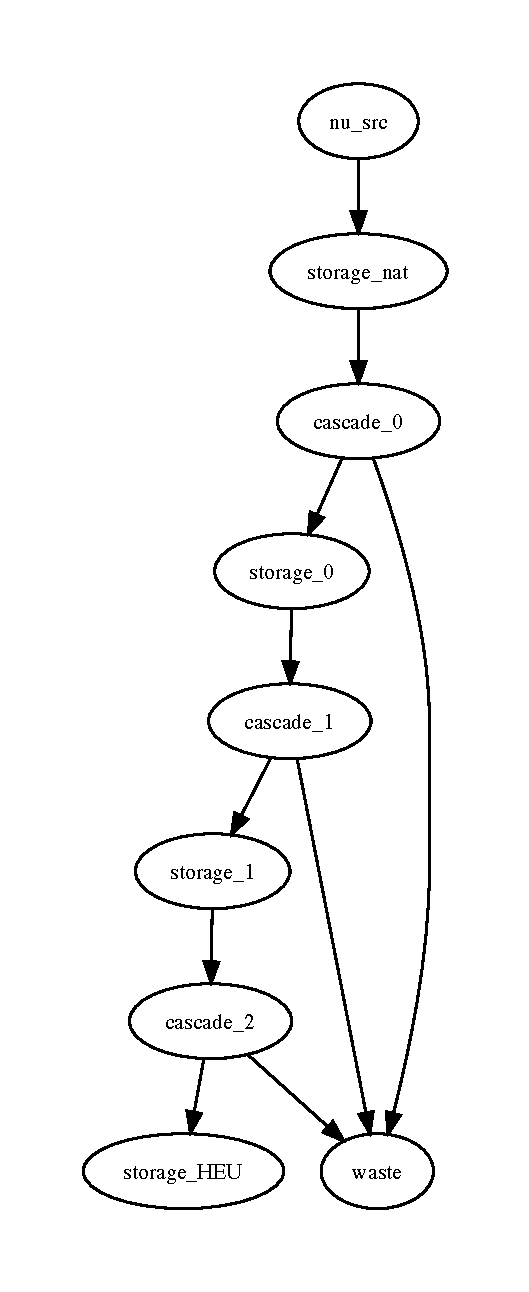
\includegraphics[scale=0.68]{flow_case_2_no_recy.pdf}
%%   \caption{Illustration of the material flow between the different level of
%%       cascades without tail recycling, in this diagram, nu\_src corresponds to
%%       an infinite source of natural uranium, cascade\_ $\{n\}$ and storage\_
%%       $\{n\}$ to the cascade and the storage getting the products of the
%%       cascades at the level $\{n\}$.}\label{fig:flow}
%% \end{figure}

%% \begin{table}[htb]
%% \centering
%%   \caption{Summary of cascade properties for each level.}
%% \begin{tabular}{cllll}
%% \toprule
%% 
%% Level   &           & Assay     &       & Machines  \\
%%         & Feed      & Product   & Feed  &           \\
%% \midrule
%% 0       & 0.0071    & 0.0413    & 0.0029 & 167       \\
%% 1       & 0.0413    & 0.2043    & 0.0173 & 169       \\
%% 2       & 0.2043    & 0.5941    & 0.0971 & 168       \\
%% 3       & 0.5941    & 0.8834    & 0.3915 & 168       \\
%% 4       & 0.8834    & 0.9735    & 0.7746 & 169       \\
%% 
%% \bottomrule
%% \end{tabular}
%% 
%%   \label{tab:cascadelvl}
%% \end{table}

%%%%%%%%%%%%%%%%%%%%%%%%%%%%%%%%%%%%%%%%%%%%%%%%%%%%%%%%%%%%%%%%%%%%%%%%%%%%%%%%
\section{Acknowledgments}
This work was funded by the Consortium for Verification Technology under
Department of Energy National Nuclear Security Administration award number
DE-NA0002534

%%%%%%%%%%%%%%%%%%%%%%%%%%%%%%%%%%%%%%%%%%%%%%%%%%%%%%%%%%%%%%%%%%%%%%%%%%%%%%%%
\bibliographystyle{ans}
\bibliography{bibliography}
\end{document}
